\documentclass[9pt]{beamer}

\usepackage[version=4]{mhchem}
\usepackage[sfdefault]{FiraSans}
\usepackage{caption}
\usepackage{float}

\usetheme{metropolis}
\setbeamertemplate{footline}{} %rimuove i numeri della slide
\addtobeamertemplate{frametitle}{}{\vspace{1em}} % increase
\addtobeamertemplate{frametitle}{}{\vspace{-3em}}

\beamertemplatenavigationsymbolsempty




\title{Sintesi di Composti d'Interesse Medico per il Trattamento del Morbo d'Alzheimer}
\author{
	Relatrice: Annamaria Deagostino
	\and
	Candidato: Lorenzo Castellino
}
\date{\center{Anno Accademico 2018-2019}}

\begin{document}

\begin{frame}
	\titlepage
\end{frame}

\begin{frame}
	\frametitle{Il Morbo d'Alzheimer in Numeri}
	Il Morbo d'Alzheimer è la prima causa di demenza a livello mondiale.
	
	Si tratta di una malattia neurodegenerativa la cui incidenza aumenta con l'avanzare dell'età.
	
	Stando al World Alzheimer Report del 2018:
	
	\begin{description}
		\item [Oggi:] 50 milioni di pazienti.
		      
		\item [2050:] 152 milioni di pazienti.
		      
	\end{description}
	
	La ricerca di una cura è una delle sfide del millennio.
\end{frame}

\begin{frame}
	\frametitle{I $\beta$-Amiloidi e il loro Ruolo}
	\bigskip
	\begin{columns}
		\begin{column}{0.5\textwidth}
			Un $\beta$-amiloide è un particolare frammento proteico insolubile non ramificato.
			
			\smallskip
			Viene originato dall'azione congiunta di tre enzimi su di una proteina denominata Amyloid Precursor Protein (APP).
		\end{column}
		\begin{column}{0.5\textwidth}
			
			\begin{figure}
				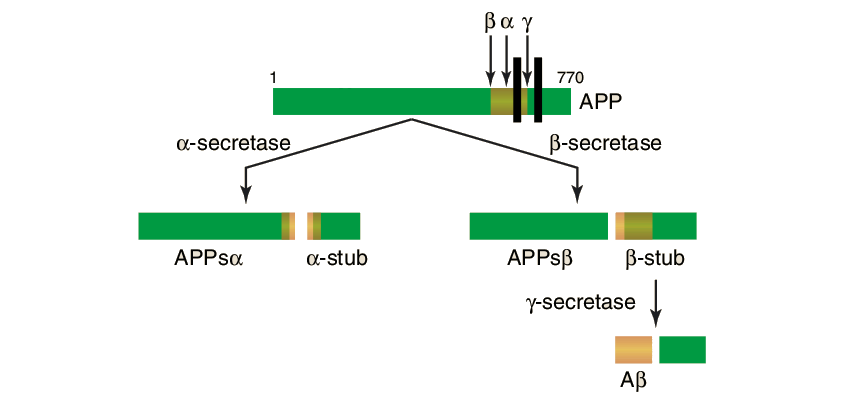
\includegraphics[width=\textwidth]{immagini/APP.png}
			\end{figure}
		\end{column}
	\end{columns}
	
	\medskip
	Si può presentare in due forme composte da 40 o 42 residui.
	
	Il frammento A$\beta$-42 se presente in anomale quantità può dare origini a fenomeni d'aggregazione con effetti nocivi per la salute.
	
\end{frame}

\begin{frame}
	\frametitle{Come Intervenire?}
	Le metodologie d'intervento studiate nel panorama della ricerca biomedica sono le più disparate.
	
	Ci soffermeremo su:
	\begin{itemize}
		\item Modulazione della neurotrasmissione.
		\item Mitigazione degli effetti di stress ossidativo.
		\item Limitazione dell'aggregazione dei A$\beta$.
	\end{itemize}
	
	
	
\end{frame}
\section{Resveratrolo}

\begin{frame}
	\frametitle{Resveratrolo: La Molecola}
	\begin{columns}
		\begin{column}{0.5\textwidth}
			Polifenolo presente in molte piante, principalmente nella vite.
		\end{column}
		\begin{column}{0.5\textwidth}
			\begin{figure}
				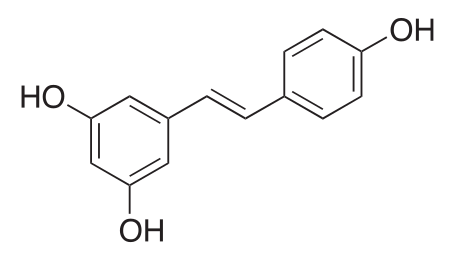
\includegraphics[width=.8\textwidth]{immagini/resveratrolo.png}
			\end{figure}
		\end{column}
	\end{columns}
	\medskip
	La sua applicazione risulta rilevante anche nel campo delle malattie neurodegenerative viste le due proprietà:
	\begin{itemize}
		\item Inibizione dell'enzima Acetilcolinesterasi (AChE).
		\item Riduzione delle specie ossidanti (ROI).
		\item Mitigazione della formazione di placche proteiche.
	\end{itemize}
\end{frame}

\begin{frame}
	\frametitle{Resveratrolo: Sintesi I}
	\begin{figure}
		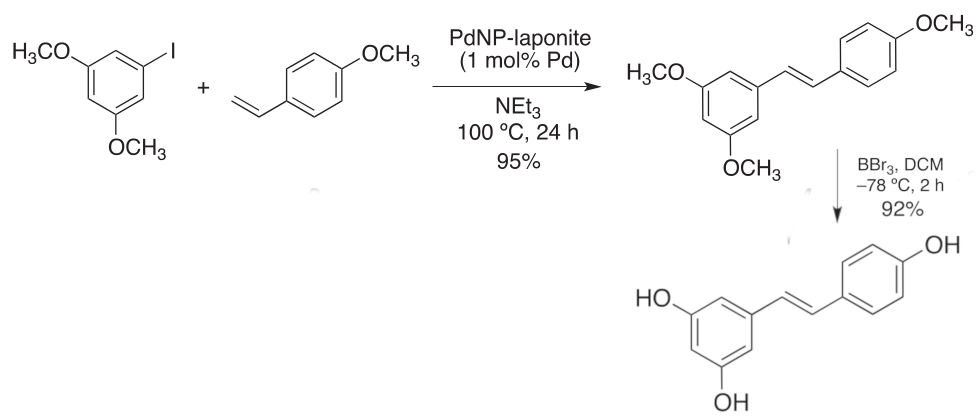
\includegraphics{immagini/totale_resveratrolo.png}
	\end{figure}
	Sintesi mediante accoppiamento Heck-Mizoroki a partire dal 1-iodo-3,5-dimetossibenzene ed il 4-metossistirene.
	
	Impiego di un catalizzatore al Palladio nanoparticellare disperso su di una resina di Laponite.
	
	Demetilazione per mezzo di \ce{BBr3} per deproteggere i gruppi idrossilici.
	
\end{frame}

\begin{frame}
	\frametitle{Resveratrolo: Sintesi II}
	\bigskip
	La reazione d'accoppiamento di Heck-Mizoroki è una reazione catalizzata da Palladio in grado di formare nuovi legami C-C a partire da un olefina e un alogenuro.
	
	\begin{figure}
		\centering
		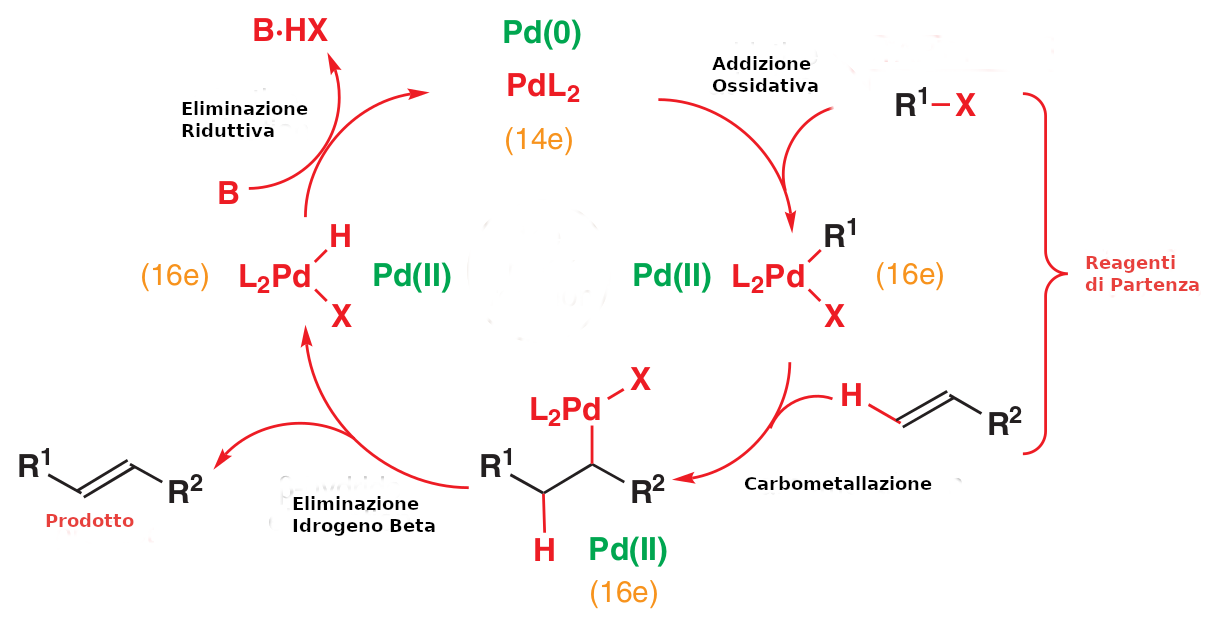
\includegraphics[width=\textwidth]{immagini/heck.png}
	\end{figure}
\end{frame}

\begin{frame}
	\frametitle{Resveratrolo: Effetti della Molecola I}
	L'azione farmacologica è stata valutata per quanto riguarda due tetrameri del Resveratrolo: Vitisina A e Heyanol A.
	
	Tramite un biotest HPLC sono stati valutati l'efficacia dell'inibizione dell'enzima AChE e la selettività per lo stesso.
	
	La diminuzione della mortalità cellulare e la diminuzione delle specie ROI in presenza di A$\beta$ sono state valutate attraverso l'osservazione di colture di cellule PC12 opportunamente trattate.
\end{frame}

\begin{frame}
	\frametitle{Resveratrolo: Effetti della Molecola II}
	
	Diminuzione della mortalità cellulare e delle specie ROI in presenza di A$\beta$ in colture di cellule PC12 opportunamente trattate.
	\begin{columns}
		\begin{column}{0.5\textwidth}
			\begin{figure}
				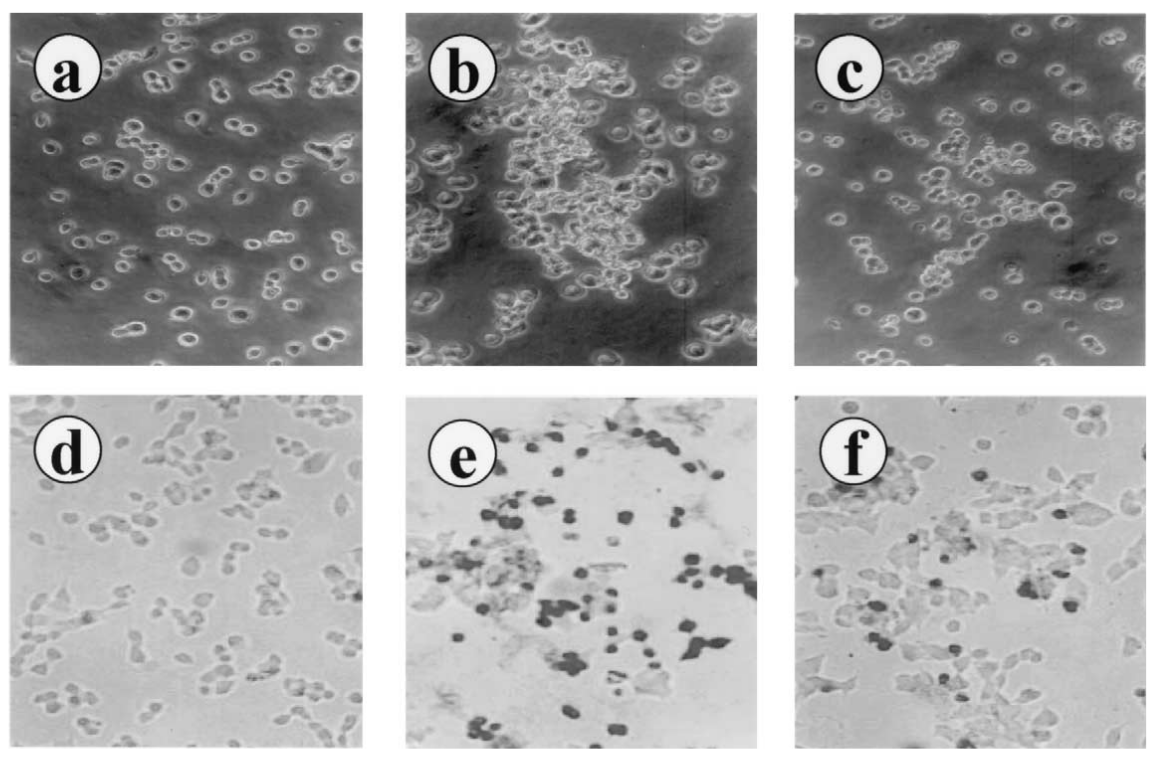
\includegraphics[width=\textwidth]{immagini/apo_resveratrolo.png}
			\end{figure}
		\end{column}
		\begin{column}{0.5\textwidth}
			\begin{figure}{t}
				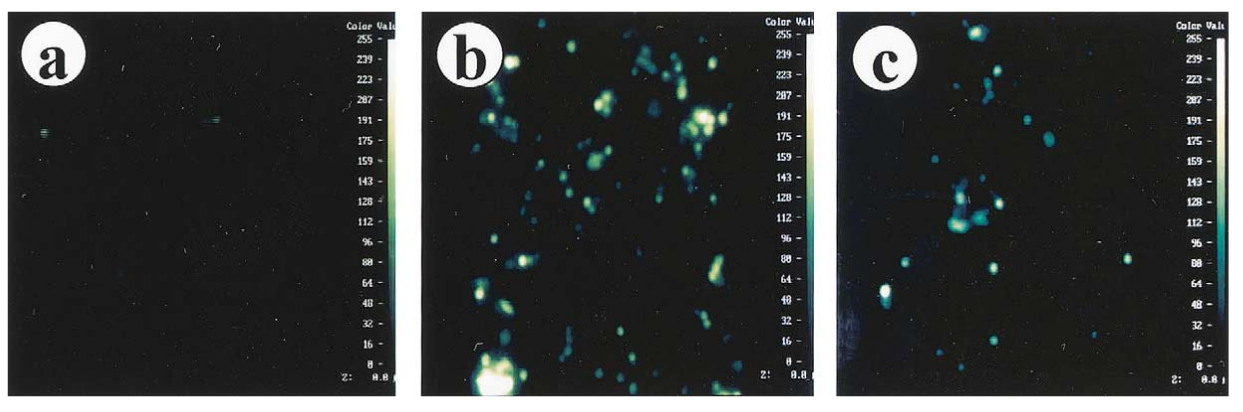
\includegraphics[width=\textwidth]{immagini/roi_resveratrolo.png}
			\end{figure}
			
		\end{column}
	\end{columns}
	\medskip
	\begin{columns}
		\begin{column}{0.5\textwidth}
			Cellule tal quale, in presenza di A$\beta$ e con l'aggiunta del Resveratrolo.
		\end{column}
		\begin{column}{0.5\textwidth}
			Immagine UV di cellule tal quale, in presenza di A$\beta$ e con l'aggiunta del Resveratrolo.
		\end{column}
	\end{columns}
	
\end{frame}

\section{Curcumina}

\begin{frame}
	\frametitle{Curcumina: La Molecola}
	\begin{columns}
		\begin{column}{.4\textwidth}
			Principale componente polifenolica del Cumino.
		\end{column}
		\begin{column}{.6\textwidth}
			\begin{figure}
				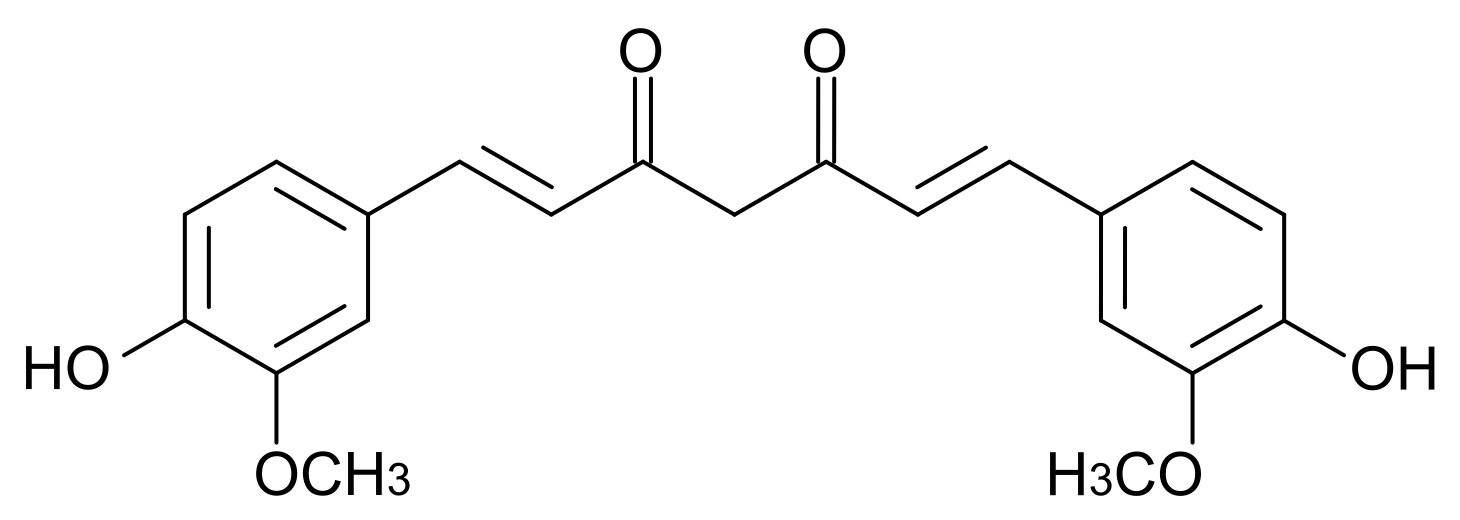
\includegraphics[width=.8\textwidth]{immagini/curcumina.png}
			\end{figure}
		\end{column}
	\end{columns}
	\bigskip
	
	Usata già nell'antica medicina cinese. L'azione medica è del tutto simile a quella già descritta per il Resveratrolo.
	
	Il principale pregio della Curcumina è la sua innata capacità di permeare la barriera emato-encefalica.
	
	Si può sfruttare questa proprietà accoppiando il farmacoforo della curcumina con quello di medicinali noti per la loro azione nei confronti dell'AD come ad esempio il Donepezil.
\end{frame}

\begin{frame}
	\frametitle{Curcumina: La Molecola II}
	\begin{figure}
		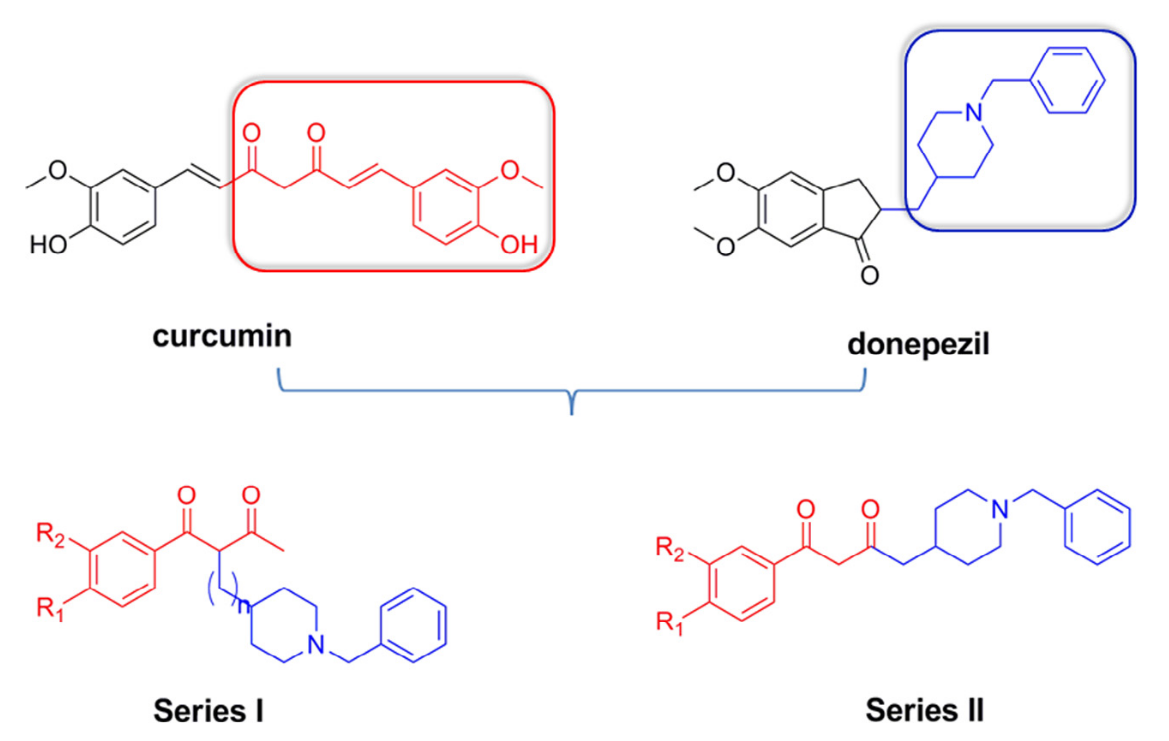
\includegraphics[scale=0.9]{immagini/generale_curcdone.png}
	\end{figure}
\end{frame}

\begin{frame}
	\frametitle{Curcumina: Sintesi I}
	A partire da reagenti commerciali sono sintetizzati i farmacofori corrispondenti per il Donepezil:
	\begin{figure}
		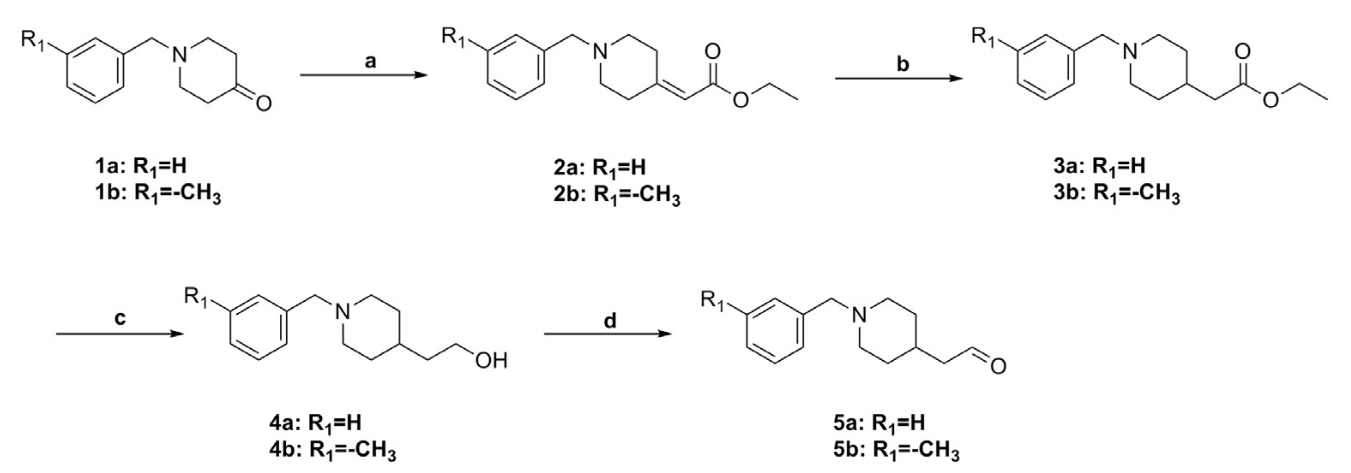
\includegraphics[width=.6\textwidth]{immagini/farmadone_curcdone.png}
	\end{figure}
	E per la Curcumina:
	\begin{figure}
		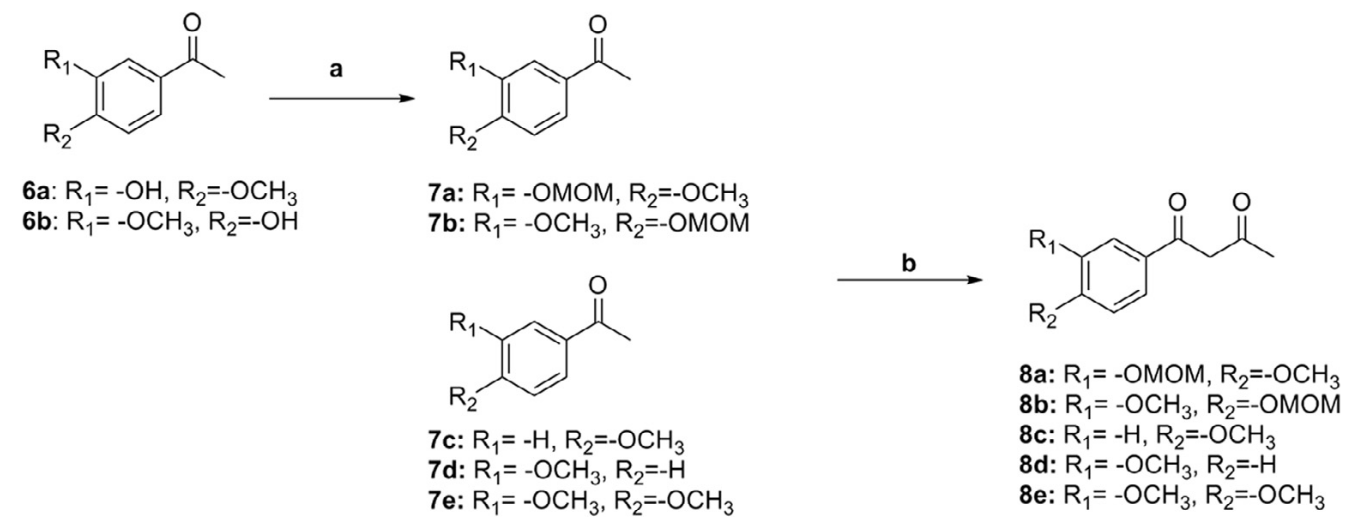
\includegraphics[width=.6\textwidth]{immagini/farmacurc_curcdone.png}
	\end{figure}
\end{frame}

\begin{frame}
	\frametitle{Curcumina: Sintesi II}
	I due farmacofori ottenuti vengono accoppiati per formare i composti desiderati della prima serie per mezzo di una condensazione aldolica:
	\begin{figure}
		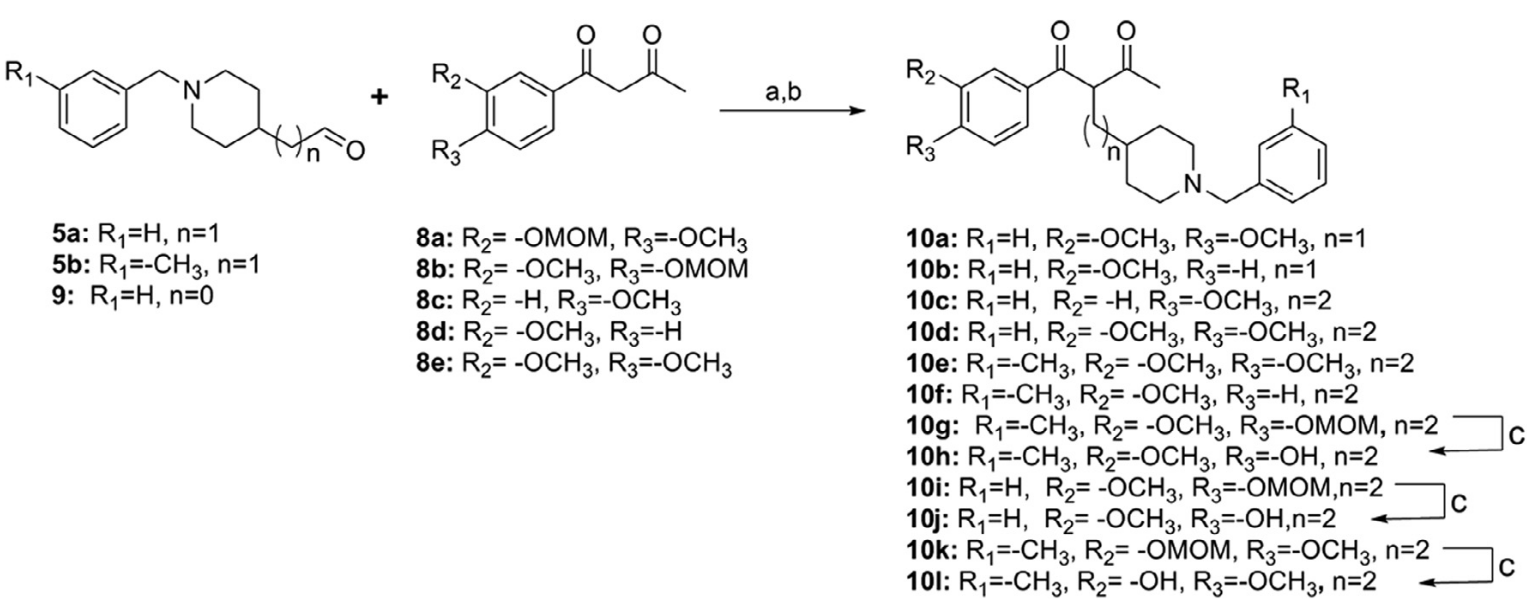
\includegraphics[width=.6\textwidth]{immagini/condserie1_curcdone.png}
	\end{figure}
	E per la seconda serie grazie ad una condensazione di Claisen:
	\begin{figure}
		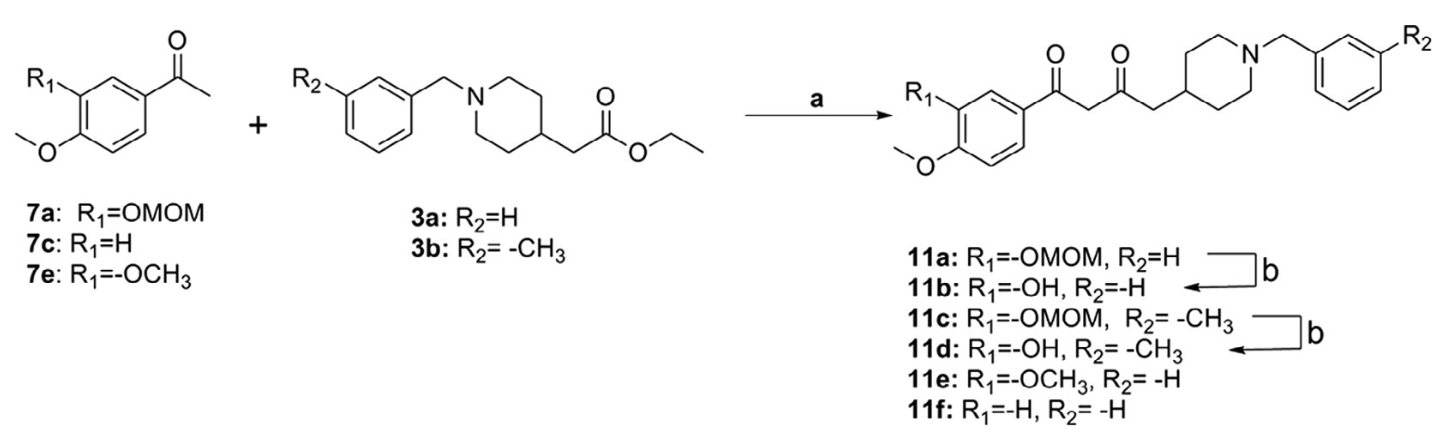
\includegraphics[width=.6\textwidth]{immagini/condserie2_curcdone.png}
	\end{figure}
\end{frame}

\begin{frame}
	\frametitle{Curcumina: Effetti della Molecola}
	
\end{frame}

\section{Bipiridine}

\begin{frame}
	\frametitle{Bipiridine: La Molecola}
\end{frame}

\begin{frame}
	\frametitle{Bipiridine: Sintesi}
\end{frame}

\begin{frame}
	\frametitle{Bipiridine: Effetti della Molecola}
\end{frame}

\section{Conclusioni}

\begin{frame}
	\frametitle{Concludendo...}
	\begin{itemize}
		\item Non si è ancora trovata una cura al Morbo d'Alzheimer
		\item La chimica organica può fornire a medici e biochimici gli strumenti per affrontare il problema: \begin{itemize}
			      \item Attraverso la sintesi di composti ispirati a prodotti 	presenti in natura come visto nelle sezioni relative a Resveratrolo e Curcumina.
			      \item Sintetizzando molecole ad hoc sulla base delle funzionalità richieste.
		      \end{itemize}
	\end{itemize}
\end{frame}


\begin{frame}
	\center{\huge{Grazie a tutti per l'attenzione!}}
\end{frame}
\end{document}
